\chapter{Diseño del entorno}



\subsection{API de \textit{PettingZoo}}

Como ya habíamos mencionado en el apartado del Estado del arte, \textit{PettingZoo} es una librería que ofrece una gran cantidad de entornos multiagente. Una de las ventajas de esta librería, es que ofrece una estructura de creación de entornos muy clara. Esta estructura es muy similar a la estructura de creación de entornos de OpenAI que ya habíamos comentado anteriormente. Seguir esta estructura en un entorno facilita el entrenamiento de agentes, ya que no es necesario modificar el código demasiado si la mayoría de entornos siguen el mismo patrón. Por esto, tal y como habíamos planteado en el apartado de Alcance, usaremos la estructura de \textit{PettingZoo} para nuestro entorno.

En primer lugar, para diseñar un entorno es necesario que tipo de entorno será. Para esto \textit{PettingZoo} provee de diferentes clases para diferentes tipos de entorno. Existen varios tipos de entorno multiagente, por ejemplo: entornos por turnos, entornos paralelos, etc. En nuestro caso, los agentes que actuaran en el juego lo harán a la vez, por lo tanto, la clase más apropiada será \textit{ParallelEnv}, diseñada para entornos donde ambos agentes actúan en paralelo.

Una vez elegida la clase a partir de la cual crearemos el entorno, faltaría diseñar unas funciones y atributos específicos, que gracias a la estructura de \textit{PettingZoo} siempre son los mismos. Las funciones y atributos que deberemos implementar son las siguientes:

\begin{itemize}
    \item Atributo \textit{observation\_ space}.
    \item Atributo \textit{action\_ space}.
    \item Atributo \textit{possible\_ agents}.
    \item Función \textit{Render}.
    \item Función \textit{Close}.
    \item Función \textit{Reset}.
    \item Función \textit{Step}.
\end{itemize}

En los siguientes apartados realizaremos una breve explicación cuál es el objetivo de cada uno de estos métodos o atributos.

\subsubsection*{Atributo \textit{observation\_ space}}

Este atributo sirve para definir que forma tendrán las observaciones que proporciona el entorno. Para definir este atributo se usa la API de OpenAI, en particular el módulo Spaces. En nuestro caso, como explicaremos más adelante, se usará una imagen RGB de dimensiones 600 x 800. Esta se representa usando la API de OpenAI como la clase Box.

\subsubsection*{Atributo \textit{action\_ space}}

Este atributo sirve para definir que forma deben tener las acciones tomadas por el agente. Al igual que con el atributo observation\_ space, se define usando la API de OpenAI. En nuestro caso, como explicaremos más tarde, usaremos una lista de diferentes valores donde cada posición de la lista codificará el uso de las diferentes acciones que puede realizar el agente en el entorno. Esta lista se representa usando la API de OpenAI como la clase MultiDiscrete.

\subsubsection*{Atributo \textit{possible\_ agents}}

Este atributo define los posibles agentes que puede tener el entorno. En nuestro caso, al principio del proyecto se limitó a únicamente 2 jugadores, pero durante la realización de este, y con la infraestructura existente, se vio que se podía permitir hasta 4 agentes sin realizar ningún cambio en el código.

\subsubsection*{Función \textit{Render}}

Esta función se encarga de mostrar de forma gráfica lo que está sucediendo en el entorno. Esto puede ser mostrando texto por la consola, creando un display de imágenes, etc. En nuestro caso, se abrirá una ventana del módulo \textit{Pygame} \cite {pygame} con la información de la última captura de pantalla realizada.

\subsubsection*{Función \textit{Close}}

Esta función se encarga de cerrar el entorno de forma segura, destruyendo los elementos que se hayan de destruir. En nuestro caso, es necesario cerrar el módulo \textit{Mss} \cite {mss}, cerrar el thread de comunicación, destruir el proceso de \textit{Xvfb} \cite {xvfb} y el proceso de \textit{Mari0}.

\subsubsection*{Función \textit{Reset}}

Esta función se encarga de rehacer el entorno de forma que sea seguro llamar a los métodos \textit{Step} y \textit{Render} sin problemas. Además debe comenzar el entorno desde el principio. En nuestro caso simplemente ejecutamos la función de \textit{Reset} implementada en el juego.

\subsubsection*{Función \textit{Step}}

Esta función se encarga de recibir las acciones de los agentes, ejecutarlas y devolver la información del entorno. En particular debe devolver para cada agente la observación del entorno, la recompensa obtenida por las acciones realizadas, el estado de finalización del entorno y alguna información adicional en caso de ser necesario.


Una vez explicado la API de PettingZoo que utilizaremos para crear nuestro entorno, pasaremos a explicar detalladamente Mari0 y sus componentes. Para facilitar las futuras explicaciones, explicaremos los elementos básicos que componen este videojuego, así como su objetivo y sus mecánicas principales.

\section{Mari0: Mario Bros con portales}

Tal y como hemos explicado anteriormente, este videojuego es la combinación entre los videojuegos Mario Bros y P0rtal. Al ser una combinación entre estos videojuegos comparte muchos de sus elementos, entre ellos sus objetivos. El objetivo de estos videojuegos es llegar al final de cada nivel. En cada nivel se proponen diferentes retos y usando los elementos del entorno disponibles y las mecánicas propias del juego, se deben resolver estos retos. El juego está limitado a 4 jugadores como máximo.

\subsection{Mecánicas}

Las mecánicas principales de este juego son el movimiento básico del Mario y la pistola de portales. El movimiento básico consiste en el movimiento a izquierda o derecha y el salto. La pistola de portales es algo más compleja. 

\subsection*{Movimiento y acciones}

El movimiento y las acciones básicas de este juego son más variadas que en juegos similares. Algunas de estas acciones no se han implementado en el entorno porque añadían demasiada complejidad al entorno o simplemente porque no aportaban ninguna ventaja. Las principales acciones que se pueden realizar son:

\begin{itemize}
    \item Movimiento: Moverse a la derecha o izquierda.
    \item Sprint: cuando se está moviendo hacia alguna dirección es posible esprintar. Esta acción no está implementada en el entorno.
    \item Salto alto: Este es el salto en el cual se llega a máxima altura. Este es el único tipo de salto que está implementado en el entorno.
    \item Salto bajo: Si una vez presionado el botón de salto, se deja de presionar, el jugador realiza un salto de menor altura. Este tipo de salto no está implementado.
    \item Usar objeto: Esta acción usa el objeto que está más cerca del jugador. Se usa principalmente para agarrar cajas y accionar pulsadores.
    \item Ataque: Esta acción solo puede usarse cuando el jugador está en el estado de Mario de fuego. El jugador suelta una bolita de fuego que rebota y daña a los enemigos que golpee. Esta acción no está implementada en el entorno.
    \item Portal 1 y 2: Con esta acción el jugador dispara su portal 1 o 2 en un ángulo desde su posición.
    \item Recargar portales: Con esta acción el jugador retira todos los portales que haya colocado.
\end{itemize}

\subsection*{Portales}

Cada jugador dispone de una pistola con dos tipos de portales, el portal izquierdo y el derecho o portales 1 y 2, cada uno representado con un color distinto. Estos portales se pueden atravesar por los todos los jugadores y por otros elementos como cajas y láseres. En la figura \ref {fig:portal} podemos ver mejor el funcionamiento de un portal.

\begin{figure}[h]
    \centering
    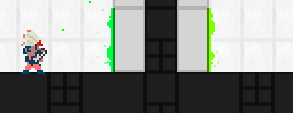
\includegraphics[width=0.9\textwidth]{img/portal-function.png}
    \caption{Funcionamiento de un portal [Elaboración Propia]}
    \label{fig:portal}
\end{figure}

Si el jugador que aparece en la figura atraviesa uno de los lados del portal, aparecerá en el otro lado del portal manteniendo la dirección del movimiento y su velocidad. Extrapolando este conocimiento, cuando un jugador atraviesa un portal, la magnitud de su velocidad se mantendrá intacta al salir por el otro lado del portal, mientras que su dirección estará dictada por la dirección en la que está enfocada el portal de salida.

Aunque los portales son una gran herramienta, también tienen sus limitaciones. Las principales limitaciones que hemos encontrado son:

\begin{itemize}
    \item Los portales solo pueden colocarse sobre superficies de color grisáceo como la que podemos ver en la figura anterior.
    \item No es posible disparar proyectiles de portales a través de un portal abierto.
    \item Cada jugador solo puede tener colocado únicamente 1 portal de cada tipo a la vez. Además, los proyectiles de los portales viajan únicamente en línea recta.
    \item Existen algunos elementos que no permiten que los proyectiles de portales los atraviesen y cuando un jugador pasa a través de estos, todos los portales colocados por este jugador se eliminan. Adicionalmente, el jugador dispone de una tecla para eliminar todos los portales colocados voluntariamente.
\end{itemize}


\subsection{Elementos del entorno}

\subsection*{Láseres azules}

Estos láseres son tangibles por los jugadores y por lo tanto pueden servir como plataforma o como obstáculo. Adicionalmente, estos láseres pueden atravesar portales dándoles mucha más utilidad. Finalmente, los proyectiles de portales pueden atravesar estos láseres sin sufrir ninguna consecuencia. En la figura \ref {fig:laser-azul} podemos ver un ejemplo de estos láseres.

\begin{figure}[h]
    \centering
    
\includegraphics[width=0.1\textwidth]{img/laser-azul.png}
    \caption{Láser azul de Mari0 [Elaboración Propia]}
    \label{fig:laser-azul}
\end{figure}

\subsection*{Láseres anti-portales}

Estos láseres son elementos que los jugadores pueden atravesar pero con ciertas consecuencias. En primer lugar, los proyectiles de portales no pueden atravesar estos láseres. Adicionalmente, cuando un jugador los atraviesa, eliminan todos los portales colocados por este jugador. Este láser es muy útil en la creación de niveles y sobre todo para prevenir situaciones extrañas donde un jugador sea teletrasportado a una parte del nivel que ya se haya superado.

\begin{figure}[h]
    \centering
    
\includegraphics[width=0.1\textwidth]{img/laser-antiportal.png}
    \caption{Láser anti-portal de Mari0 [Elaboración Propia]}
    \label{fig:antiportal}
\end{figure}

\subsection*{Elementos accionadores}

Dentro del entorno existen varios elementos que se pueden accionar, desencadenando así una reacción. Los elementos más comunes son botones y pulsadores. Los primeros se accionan cuando tienen un jugador o una caja encima de ellos mientras que los últimos se accionan mediante la tecla de uso del jugador. Ambos disponen a su vez de una línea que sirve para indicar que elemento accionan. Podemos ver ejemplos de estos elementos en la figura \ref {fig:boton}.

\begin{figure}[h]
    \centering
    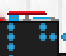
\includegraphics[width=0.1\textwidth]{img/boton.png}
    
\includegraphics[width=0.05\textwidth]{img/pulsador.png}
    \caption{Botón y pulsador de Mari0 [Elaboración Propia]}
    \label{fig:boton}
\end{figure}

Además de estos elementos que hemos explicado, existen muchos otros como los geles, cajas, láseres rojos, palancas de salto, láseres anti-gravitatorios etc. El objetivo de este apartado no es explicar todos los elementos que existen sino solo los principales. Con los elementos que hemos explicado hasta ahora es suficiente para continuar nuestra explicación del diseño del entorno. 



Una vez explicado los elementos del videojuego, pasaremos a explicar las diferentes tareas que tuvimos que realizar para el funcionamiento del entorno. En primer lugar, era necesario realizar un diseño que nos permitiera cumplir los objetivos propuestos. La primera tarea a realizar fue encontrar un mapa para 2 jugadores como mínimo.

\subsection{Mapa cooperativo}
Mari0 es un juego opensource desarrollado por la comunidad. Este juego obtuvo mucha popularidad en los años 2012 a 2015. Durante esta epoca se creo un foro sobre el juego donde cualquier diseñador interesado podía enviar una copia de su mapa para que el resto de los jugadores del juego pudieran valorarlo. El juego ya trae varios mapas creados por los creadores del juego. Todos estos mapas pueden jugarse con más de 1 jugador, pero solo es necesario 1 jugador para completarlos. Aún así, ninguno de estos es estaba completamente diseñado para un minimo 2 o más jugadores.

En nuestro caso es necesario un mapa diseñado para 2 jugadores como minimo. Por ello teniamos 2 opciones. La primera opcion consistía en implementar el mapa nosotros mismos. Esta tarea no es demasiado dificil ya que el juego trae consigo un editor de niveles muy intuitivo y facil de usar. Aún así, esta tarea no estaba prevista y aún ser sencilla, es necesario un tiempo para desarrollar y testear el mapa. La otra opcion consistia en realizar una busqueda por el foro \cite{mari0-forum} con el objetivo de encontrar algún mapa que cumpliera estas características. 

Decidimos buscar en el foro y en caso de encontrar un mapa, analizar si era viable usarlo como el mapa pricipal del entorno. En caso de no encontrar ninguno viable, habría que implementarlo desde 0. Para facilitar la busqueda, se contacto con el usuario HugoBDesigner, un diseñador muy popular de mapas de Mari0, ya que este se dedicaba a realizar valoraciónes de los mapas que le enviaban otros usuarios y colaboraba activamente con los creadores del videojuego. Este diseñador colaboró con la busqueda aportadonos enlaces a 3 mapas cooperativos que él había jugado durante la epoca del 2012. De estos 3 enlaces, solo 1 permanecía activo. Este mapa llamado Bowser Cooperative Testing Initiative fue el que usamos para como mapa principal para el entorno. El mapa puede descargarse de \cite {mari0-mapa} gracias al diseñador Pixel Worker. 

Para comprobar que el entorno no puede ser resuleto por un solo agente usaremos la figura \ref {fig:mapa} que es el principio del primer nivel del mapa.

\begin{figure}[ht]
    \centering
    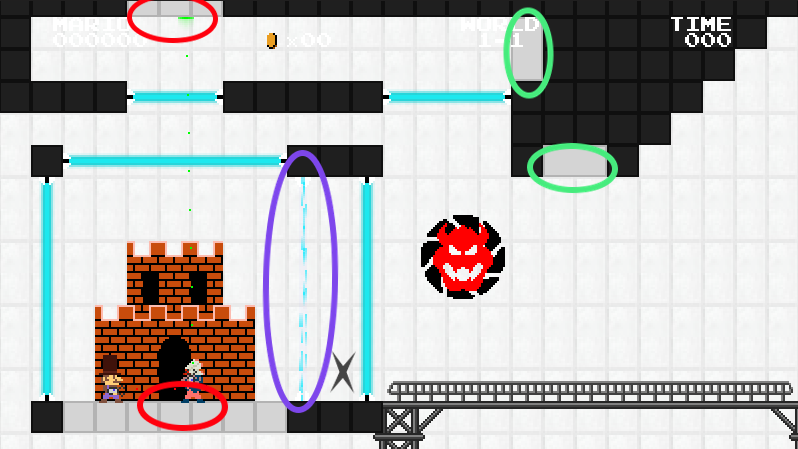
\includegraphics[width=0.9\textwidth]{img/mario-1-level.png}
    \caption{Nivel del mapa Bowser Cooperative Testing Initiative \cite {mari0-mapa}}
    \label{fig:mapa}
\end{figure}

La forma de resolver este nivel es la siguiente:
\begin{itemize}
    \item Paso 1: En primer lugar, uno de los dos jugadores, de ahora en adelante jugador 1, debe colocar un portal en cada uno de los circulos rojos indicados en la figura. Con este movimiento se consigue que el jugador 1 pase a la sección superior.
    \item Paso 2: El jugador 2 debe colocarse donde se encuentra la X indicada en la figura. Desde esta posicion debe disparar dos portales a los circulos verdes indicados en la figura. Con este paso el jugador 1, que se encuentra en la sección superior, será capaz de atravesar estos portales y pasar fuera del cuadrilatero inicial.
    \item Paso 3: Una vez el jugador 1 se encuentra fuera del cuadrialtero, el jugador 2 debera realizar las misma acciónes que el jugador 1 en el primer paso.
    \item Paso 4: Mientras eso ocurre, el jugador 1 deberá colocar sus portales donde los colocó el jugador 2 en el paso 2.
    \item Si se han realizado correctamente todos los pasos, ambos jugadores deberian haber salido del cuadrialtero inicial.
\end{itemize}

Es facilmente visible que un solo jugador no puede completar este primer nivel. Esto se debe a que desde la sección superior es imposible colocar los portales donde debe para salir del cuadrilatero. El resto de niveles del mapa incluyen este tipo de puzles los cuales, al igual que este, necesitan como minimo 2 agentes para ser resueltos.

Una vez encontrado el mapa, debíamos decidir como estarían codificadas las acciones de los agentes y las observaciones usando la API de OpenAI.

\subsection{Acciones}

En el apartado de Mari0: Mario Bros con portales explicamos las diferentes acciones que un jugador podia executar en el juego base. Aunque estas acciones tienen sentido cuando el juego se utiliza por personas, algunas de estas no aportan ningun valor para el entorno. 

Asi que una de las acciones fue decidir cuales acciones de todas las posible se quedarían en el entorno. Para selecionar estas acciones se analizo cual era el conjunto minimo de acciones necesarias para resolver el mapa del entorno. Estas acciones correspondian a moverse a izquierda y derecha, salto alto, usar objeto, disparar portales 1 y 2 y recargar portales. La accion de salto bajo no añade ninguna mejora al set de movimiento, ya que no hay ninguna ventaja en hacer un salto de menor tamaño. Y la accion de atacar tampoco se utiliza en el mapa ya que el jugador nunca llega al estado de Mario de fuego.

La siguiente tarea era decidir como se codificarian estas operaciones en la API de OpenAI. Todas las operaciones deberían tener la posibilidad de no ser ejecutadas. Nos dimos cuenta que era posible codificar todas las acciones usando numeros enteros. La codificación de las acciones fue la siguiente:

\begin{itemize}
	\item Si el valor de la accion es 0 significa que no debe ejecutarse.
	\item Para acciones de una sola variante como Saltar y Recargar portales, el valor 1 significa ejecutar esa accion.
 	\item Para la accion de Usar objeto, la orientación del personaje importa, por los tanto era necesario dar la posibilidad de usar un objeto a la derecha o a la izquierda del jugador. Por lo tanto el valor 1 simboliza coger un objeto a la izquierda del jugador y 2 un objeto a la derecha.
	\item Para la accion de movimiento a ambos lados el valor 1 codifica movimiento a izquierda y el valor 2 a derecha.
	\item Para las acciones de disparar portal 1 y disparar portal 2, cualquier valor diferente a 0 indica el angulo con respecto al jugador en el que se debe disparar el portal.
\end{itemize}

Cada accion tiene una posicion especifica en la lista. Por ejemplo, la lista de acciones podria verse como en la tabla \ref {tab:accion}. Esta lista codificaría que el jugador se esta moviendo para la izquierda mientras realiza un salto y dispara el portal 1 con un angulo de 15 grados.

\begin{table}[h]
	\begin{center}
		\begin{tabular}{| l | l | l | l | l | l |}
			\hline
			\textbf{Movimiento} & \textbf{Salto} & \textbf{Usar} & \textbf{Recargar} & \textbf{Portal 1} & \textbf{Portal 2} \\ \hline
			1                   & 1              & 0             & 0                 & 15                & 0                 \\ \hline
		\end{tabular}
		\caption{Ejemplo de set de acciones de un agente[Elaboración propia]}
		\label{tab:accion}
	\end{center}
\end{table}


En otros juegos similares se suele escoger una codificacion más simple, donde todas las acciones simples se juntan en una unica posicion. En nuestro caso no decidimos usar esta codificacion ya que queriamos permitir que las acciones se ejecutaran al mismo tiempo. Aun asi, la accion de moverse hacia derecha o izquierda se ha unido en una sola posicion ya que son acciones complementarias.

\subsection{Tipo de observaciones}
La siguiente tarea a realizar era decidir que tipo de obsevaciones extraeriamos del entorno. Tal y como habiamos explicado en el apartado de Definición de conceptos, los agentes necesitan conocer el estado del entorno para poder aprender y tomar sus acciones. Para ello es necesario obtener una observación del juego. 

Existen dos principales formas de obtener el estado del juego: Serializando alguna clase que contenga los pricipales elementos del juego o simplemente capturar la imagen producida por el videojuego. La primera alternativa se suele usar en entornos más simples donde los elementos importantes para entrenar son pocos y facilmente serializables. Un ejemplo de este tipo de entornos puede ser el entorno Level-Based Foraging visto en el apartado Estado del arte. En este entorno simplemente se pasa una cuadricula con los elementos que hay en cada una de ellas. Podemos ver la representación del entorno en la figura \ref {fig:foraging-2}.

\begin{figure}[h]
    \centering
    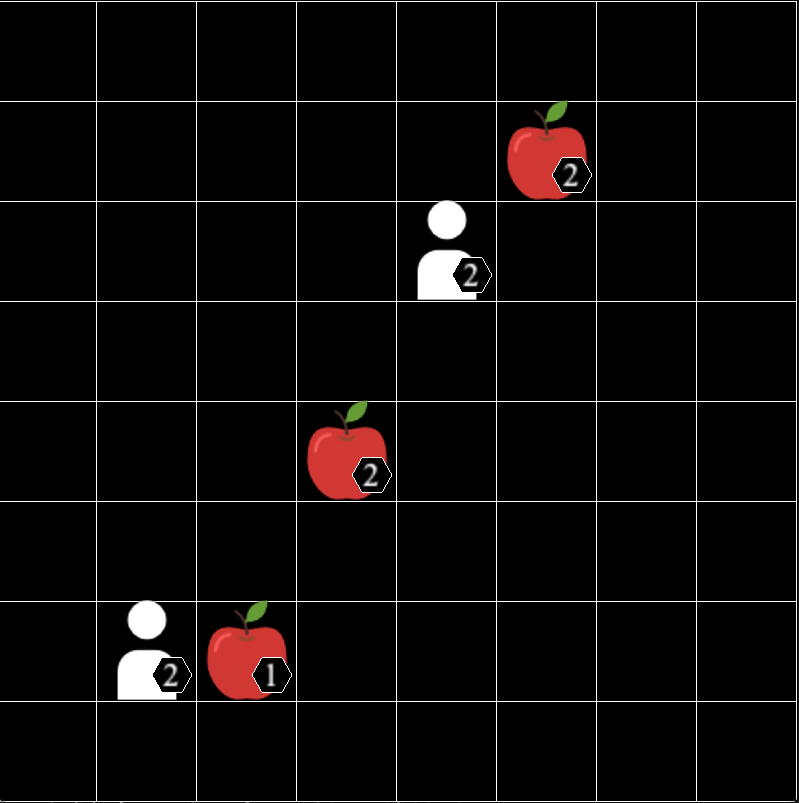
\includegraphics[width=0.3\textwidth]{img/level-base.png}
    \caption{Entorno gráfico de Level-Based Foraging \cite {env-list}}
    \label{fig:foraging-2}
\end{figure}

La segunda alternativa suele ser usada en entornos más complejos donde serializar todos los elementos es realmente complejo. Un ejemplo que utiliza esta alternativa es el entorno MALMÖ.

Nuestro entorno no es lo suficientemente simple para poder usar la primera opcion. Esto se debe los elementos importantes para el entrenamiento de un agente en nuestro entorno son muchos, muy variados y dificilmente serializables. Tomemos por ejemplo la figura \ref {fig:observartion} que forma parte de uno de los primeros niveles del mapa. 

\begin{figure}[h]
    \centering
    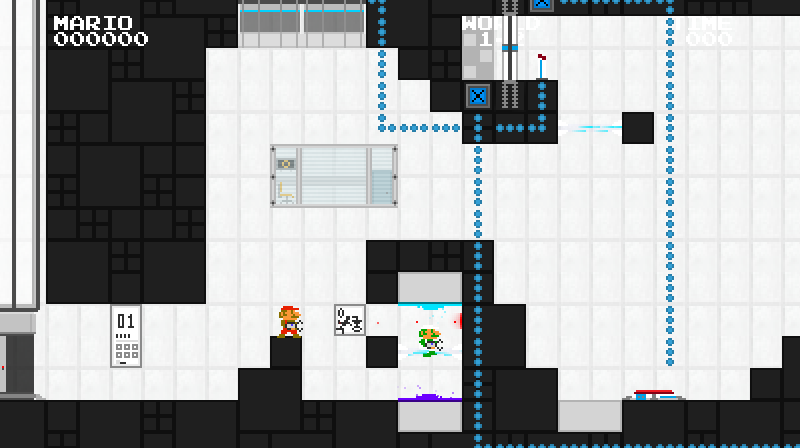
\includegraphics[width=0.9\textwidth]{img/BCTI_observation.png}
    \caption{Nivel del mapa Bowser Cooperative Testing Initiative \cite {mari0-mapa}}
    \label{fig:observartion}
\end{figure}

Esta sería la lista de elementos que deberíamos serializar para el entorno en caso de usar la primera alternativa:

\begin{itemize}
    \item Todos los bloques donde los jugadores pueden golpearse, incluyendo el techo del mapa. Esto es asi ya que gracias a los portales estos bloques pueden ser obstaculos o tener un papel relevante en el nivel.
    \item La posicion de los jugadores.
    \item La posicion de botones, pulsadores, palancas de salto, dispensadores de gel, puertas y dispensadores de cajas. Y además incluir la relación de que elementos accionan cada boton, pulsador etc.
    \item Todos los bloques donde los jugadores pueden colocar portales.
    \item Lasers azules, lasers rojos y lasers de destruccion de portales.
    \item Partes acuaticas o de acido.
    \item Enemigos y elementos dañinos.
\end{itemize}

Serializar esto es una tarea complicada y más aun teniendo en cuenta que los modulos del sistema no estan diseñados para esto. Si el juego se hubiera diseñado con la idea de pasar todos estos elementos a otro programa, esta sería una opcion viable. Pero en nuestro caso, esta opcion requeriría reconstuir practicamente todo el juego, algo impracticable. De modo que la unica opcion que queda es capturar las imagenes producidas por el videojuego y enviarlas a los agentes. Para esto, se decidio utilizar la resolución base del videojuego (600 x 800) y obtener sus imagenes en formato RGB. Por lo tanto, el tamaño de la observación sería 800 * 600 * 3 * 255.

Una vez diseñada la codificación de las observaciones y las acciones, la siguiente tarea consistía en diseñar un sistema para capturar el output del juego y pasarlo a los agentes.



